\documentclass[12pt]{article}
\usepackage[paperwidth=15.5cm, paperheight=16.5cm, margin=0.2cm]{geometry}
\usepackage{tikz}
\usetikzlibrary{positioning, arrows.meta, calc, decorations.pathreplacing}
\pagestyle{empty}
\setlength{\parindent}{0pt}

% ============================================================================
% COLORES Y ESTILOS
% ============================================================================
\definecolor{pastelblue}{RGB}{230, 242, 252}

\tikzset{
  box/.style={
    draw, thick, fill=pastelblue,
    minimum height=1.5cm,
    minimum width=2cm,
    font=\small\sffamily,
    align=center
  },
  ffbox/.style={
    draw, thick, fill=pastelblue,
    minimum width=3.6cm, 
    minimum height=2cm,
    font=\small\sffamily,
    align=center
  },
  signal/.style={-{Stealth[length=2mm]}, thick, black}, 
  wirelabel/.style={font=\tiny\sffamily, text=black, midway, above}
}

% Extend macro
\newcommand{\drawextend}[3]{
  \draw[thick, fill=pastelblue] 
    (#1-1.2, #2+0.3) -- 
    (#1+1.2, #2+0.6) -- 
    (#1+1.2, #2-0.6) -- 
    (#1-1.2, #2-0.3) -- cycle;
  \node[font=\small\sffamily] (#3) at (#1, #2) {Extend};
  \coordinate (#3_in) at (#1-1.2, #2);
  \coordinate (#3_out) at (#1+1.2, #2);
}

\begin{document}
\noindent
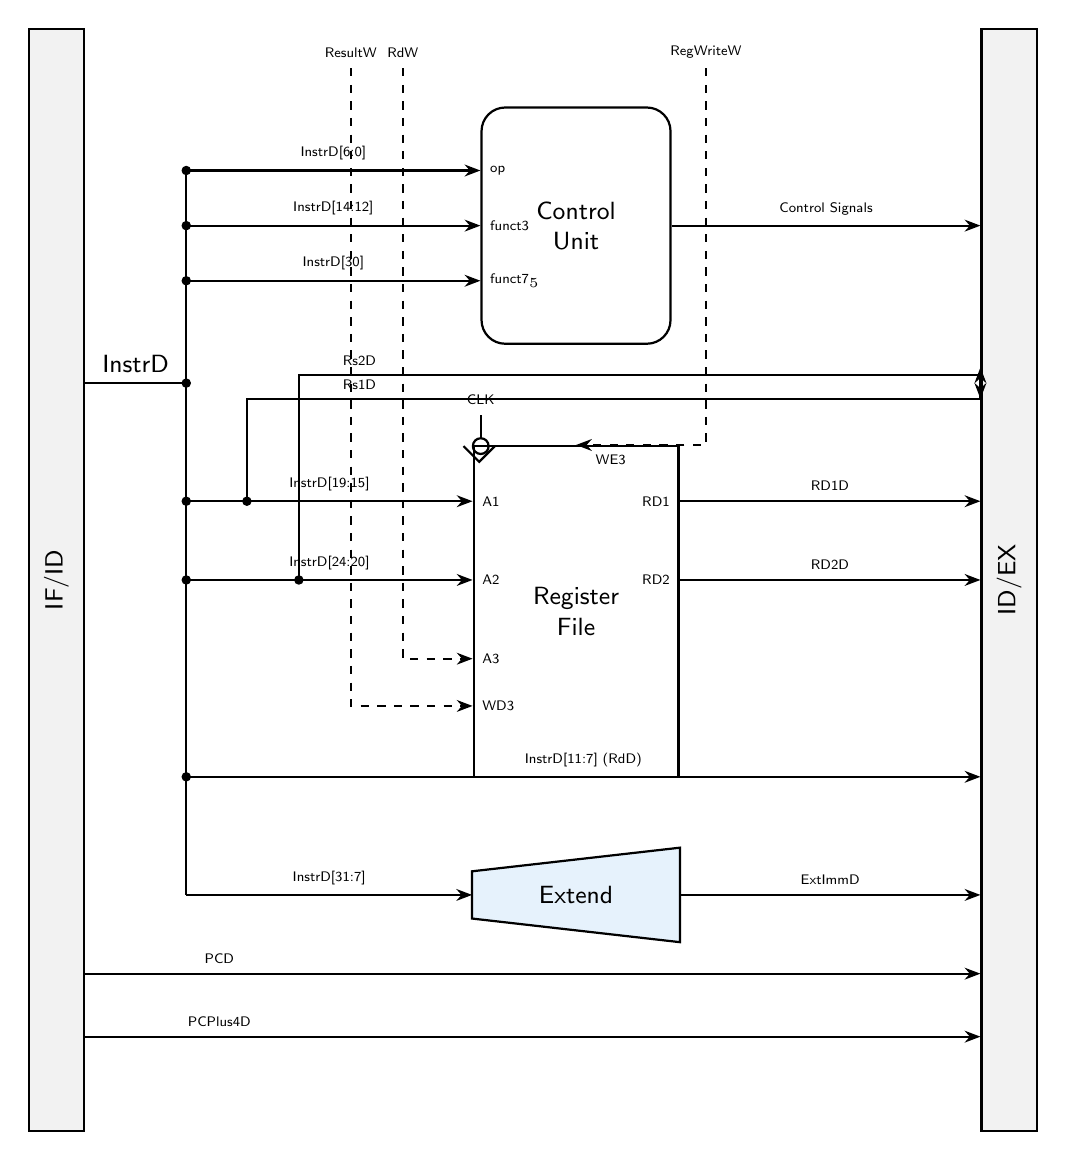
\begin{tikzpicture}[
  x=1.1cm, y=1.0cm,
  signal/.style={-{Stealth[length=2mm]}, thick, black},
  lbl/.style={font=\tiny\sffamily, text=black},
  lblcenter/.style={font=\small\sffamily, align=center},
]

% IF/ID y ID/EX Pipeline Registers
\node[draw, fill=gray!10, thick, minimum width=0.7cm, minimum height=14cm, font=\small\sffamily] (ifid_reg) at (0, 0) {\rotatebox{90}{IF/ID}};
\node[draw, fill=gray!10, thick, minimum width=0.7cm, minimum height=14cm, font=\small\sffamily] (idex_reg) at (11, 0) {\rotatebox{90}{ID/EX}};

% Componentes
% Control Unit
\node[draw, thick, fill=white, rounded corners=3mm, minimum height=3.0cm, minimum width=2.4cm, font=\small\sffamily, align=center] (ctrl) at (6.0, 4.5) {Control\\Unit};
\node[font=\tiny\sffamily, right] at (ctrl.west |- {0,5.2}) {op};
\node[font=\tiny\sffamily, right] at (ctrl.west |- {0,4.5}) {funct3};
\node[font=\tiny\sffamily, right] at (ctrl.west |- {0,3.8}) {funct7$_5$};

% Register File
\node[draw, thick, fill=white, minimum height=4.2cm, minimum width=2.6cm] (regfile) at (6.0, -0.4) {};
\node[lblcenter] at (6.0, -0.4) {Register\\File};
\node[font=\tiny\sffamily, right] at (regfile.west |- {0, 1.0}) {A1};
\node[font=\tiny\sffamily, right] at (regfile.west |- {0, 0.0}) {A2};
\node[font=\tiny\sffamily, right] at (regfile.west |- {0, -1.0}) {A3};
\node[font=\tiny\sffamily, right] at (regfile.west |- {0, -1.6}) {WD3};
\node[font=\tiny\sffamily, left]  at (regfile.east |- {0, 1.0}) {RD1};
\node[font=\tiny\sffamily, left]  at (regfile.east |- {0, 0.0}) {RD2};
\node[font=\tiny\sffamily, below] at (regfile.north -| {6.4, 0}) {WE3};

% Clock pin
\draw[thick] (4.9, 1.7) circle (1mm);
\draw[thick] (4.9, 1.8) -- ++(0, 3mm) node[above, font=\tiny\sffamily] {CLK};
\draw[thick] (4.7, 1.7) -- ++(2mm, -2mm) -- ++(2mm, 2mm);

% Extend
\drawextend{6.0}{-4.0}{ext}

% Tronco principal InstrD
\draw[thick, black] (ifid_reg.east |- {0,2.5}) -- (1.5, 2.5) node[midway, above, text=black, font=\small\sffamily] {InstrD};
\draw[thick, black] (1.5, 5.2) -- (1.5, -4.0);
\draw[fill=black] (1.5, 2.5) circle (1.5pt);

% Conexiones desde el tronco hacia Control Unit
\draw[signal] (1.5, 5.2) -- (ctrl.west |- {0,5.2}) node[lbl, midway, above] {InstrD[6:0]};
\draw[fill=black] (1.5, 5.2) circle (1.5pt);
\draw[signal] (1.5, 4.5) -- (ctrl.west |- {0,4.5}) node[lbl, midway, above] {InstrD[14:12]};
\draw[fill=black] (1.5, 4.5) circle (1.5pt);
\draw[signal] (1.5, 3.8) -- (ctrl.west |- {0,3.8}) node[lbl, midway, above] {InstrD[30]};
\draw[fill=black] (1.5, 3.8) circle (1.5pt);

% Conexiones desde el tronco hacia RegFile
\draw[signal] (1.5, 1.0) -- (regfile.west |- {0,1.0}) node[lbl, midway, above] {InstrD[19:15]};
\draw[fill=black] (1.5, 1.0) circle (1.5pt);
\draw[signal] (1.5, 0.0) -- (regfile.west |- {0,0.0}) node[lbl, midway, above] {InstrD[24:20]};
\draw[fill=black] (1.5, 0.0) circle (1.5pt);

% Conexiones desde el tronco hacia ID/EX y Extend
\draw[signal] (1.5, -2.5) -- (idex_reg.west |- {0,-2.5}) node[lbl, midway, above] {InstrD[11:7] (RdD)};
\draw[fill=black] (1.5, -2.5) circle (1.5pt);
\draw[signal] (1.5, -4.0) -- (ext_in) node[lbl, midway, above] {InstrD[31:7]};

% Cables de Bypass (Rs1D, Rs2D)
\draw[fill=black] (2.2, 1.0) circle (1.5pt);
\draw[signal] (2.2, 1.0) |- (2.2, 2.3) -- (10.4, 2.3) -| (idex_reg.west |- {0, 2.7});
\node[lbl, above] at (3.5, 2.3) {Rs1D};

\draw[fill=black] (2.8, 0.0) circle (1.5pt);
\draw[signal] (2.8, 0.0) |- (2.8, 2.6) -- (10.4, 2.6) -| (idex_reg.west |- {0, 2.3});
\node[lbl, above] at (3.5, 2.6) {Rs2D};

% Conexiones directas desde IF/ID
\draw[signal] (ifid_reg.east |- {0,-5.0}) -- (idex_reg.west |- {0,-5.0}) node[lbl, pos=0.15, above] {PCD};
\draw[signal] (ifid_reg.east |- {0,-5.8}) -- (idex_reg.west |- {0,-5.8}) node[lbl, pos=0.15, above] {PCPlus4D};

% Conexiones de salida de componentes a ID/EX
\draw[signal] (ctrl.east |- {0,4.5}) -- (idex_reg.west |- {0,4.5}) node[lbl, midway, above] {Control Signals};
\draw[signal] (regfile.east |- {0,1.0}) -- (idex_reg.west |- {0,1.0}) node[lbl, midway, above] {RD1D};
\draw[signal] (regfile.east |- {0,0.0}) -- (idex_reg.west |- {0,0.0}) node[lbl, midway, above] {RD2D};
\draw[signal] (ext_out) -- (idex_reg.west |- ext_out) node[lbl, midway, above] {ExtImmD};

% Conexiones hacia Register File (desde Writeback - desde arriba)
\draw[signal, dashed] (3.4, 6.5) node[above, lbl] {ResultW} -- (3.4, -1.6) -- (regfile.west |- {0,-1.6});
\draw[signal, dashed] (4.0, 6.5) node[above, lbl] {RdW} -- (4.0, -1.0) -- (regfile.west |- {0,-1.0});
\draw[signal, dashed] (7.5, 6.5) node[above, lbl] {RegWriteW} -- (7.5, 2.2) |- (regfile.north);

\end{tikzpicture}
\end{document}
